%%%%%%%%%%%%%%%%%%%%%%%%%%%%%%%%%%%%%%%%%%%%%%%%

% Specify the command that you want into the header of the
% index.md file

%%%%%%%%%%%%%%%%%%%%%%%%%%%%%%%%%%%%%%%%%%%%%%%%

% Options for packages loaded elsewhere
\PassOptionsToPackage{unicode}{hyperref}
\PassOptionsToPackage{hyphens}{url}
\PassOptionsToPackage{dvipsnames,svgnames*,x11names*}{xcolor}
%
\documentclass[
  12pt,
  oneside]{report}
%%\usepackage{lmodern}
%
% Set line spacing
\usepackage{setspace}
\setstretch{1.5}

\usepackage{amssymb,amsmath}
\usepackage{ifxetex,ifluatex}
\ifnum 0\ifxetex 1\fi\ifluatex 1\fi=0 % if pdftex
  \usepackage[T1]{fontenc}
  \usepackage[utf8]{inputenc}
  \usepackage{textcomp} % provide euro and other symbols
\else % if luatex or xetex
  \usepackage{unicode-math}
  \defaultfontfeatures{Scale=MatchLowercase}
  \defaultfontfeatures[\rmfamily]{Ligatures=TeX,Scale=1}
\fi
% Use upquote if available, for straight quotes in verbatim environments
\IfFileExists{upquote.sty}{\usepackage{upquote}}{}
\IfFileExists{microtype.sty}{% use microtype if available
  \usepackage[]{microtype}
  \UseMicrotypeSet[protrusion]{basicmath} % disable protrusion for tt fonts
}{}
\makeatletter
\@ifundefined{KOMAClassName}{% if non-KOMA class
  \IfFileExists{parskip.sty}{%
    \usepackage{parskip}
  }{% else
    \setlength{\parindent}{0pt}
    \setlength{\parskip}{6pt plus 2pt minus 1pt}}
}{% if KOMA class
  \KOMAoptions{parskip=half}}
\makeatother
\usepackage{xcolor}
\IfFileExists{xurl.sty}{\usepackage{xurl}}{} % add URL line breaks if available
\IfFileExists{bookmark.sty}{\usepackage{bookmark}}{\usepackage{hyperref}}
\hypersetup{
  pdfauthor={François Leroy, PhD student at CZU},
  colorlinks=true,
  linkcolor=Blue,
  filecolor=Blue,
  citecolor=Blue,
  urlcolor=Blue,
  pdfcreator={LaTeX via pandoc}}
\urlstyle{same} % disable monospaced font for URLs

%% Package geometry
\usepackage[left = 2cm,right = 2cm,top = 2cm,bottom = 2cm]{geometry}
\usepackage{pdflscape}


\usepackage{longtable,booktabs}
% Correct order of tables after \paragraph or \subparagraph
\usepackage{etoolbox}
\makeatletter
\patchcmd\longtable{\par}{\if@noskipsec\mbox{}\fi\par}{}{}
\makeatother
% Allow footnotes in longtable head/foot
\IfFileExists{footnotehyper.sty}{\usepackage{footnotehyper}}{\usepackage{footnote}}
\makesavenoteenv{longtable}
\setlength{\emergencystretch}{3em} % prevent overfull lines
\providecommand{\tightlist}{%
  \setlength{\itemsep}{0pt}\setlength{\parskip}{0pt}}
\setcounter{secnumdepth}{5}
%%% Complete the preamble of the LaTeX template
%%%------------------------------------------------------------------------------

%% Bug de bookdown: ne traite plus la déclaration "otherlangs" dans le préambule
% Pour charger les langues, écriture ici en dur du produit de bookdown
% Corrigé le 22/11/2019. A retester régulièrement: supprimer ces lignes si la compilation fonctionne sans elles.
\usepackage{polyglossia}
  \setmainlanguage[variant=american]{english}
  \setotherlanguage[]{french}
% Bug persistant le 28/02/2020

% Advised with polyglossia and babel
\usepackage{csquotes}

% Environnement "Essentiel" en début de chapitre
\usepackage[tikz]{bclogo}
\newenvironment{Essentiel}
  {\begin{bclogo}[logo=\bctrombone, noborder=true, couleur=lightgray!50]{L'essentiel}\parindent0pt}
  {\end{bclogo}}

%% Package fontspec
\usepackage{fontspec}
\setmainfont{calibri}[
  Path           = ./fonts/,
  Extension      = .ttf,
  BoldFont       = calibrib,
  ItalicFont     = calibrili,
  BoldItalicFont = calibriz]

% Rename chapters
% Below, scrpit to prevent the "chapter n" and the space use for it to
% be displayed
\usepackage{titlesec}
\titleformat{\chapter}   
{\Huge}{\thechapter{. }}{0pt}{\Huge}
%{\thechapter{. }}
\titlespacing*{\chapter}{0pt}{-50pt}{10pt}
% -50 is to up the title and 10 is the space with the text below
\usepackage{booktabs}
\usepackage{longtable}
\usepackage{array}
\usepackage{multirow}
\usepackage{wrapfig}
\usepackage{float}
\usepackage{colortbl}
\usepackage{pdflscape}
\usepackage{tabu}
\usepackage{threeparttable}
\usepackage{threeparttablex}
\usepackage[normalem]{ulem}
\usepackage{makecell}
\usepackage{xcolor}
\ifluatex
  \usepackage{selnolig}  % disable illegal ligatures
\fi
\usepackage[]{natbib}
\bibliographystyle{apa}

\author{François Leroy, PhD student at CZU}
\date{2021-08-25}

% to include pdf
\usepackage{pdfpages}



%%%%%%%%%%%%%%%%%%%%%%%%%%%%%%%%%%%%%%%%%%%%%%%%%%%%%%%%%%%%%
% Start of the documents
\begin{document}

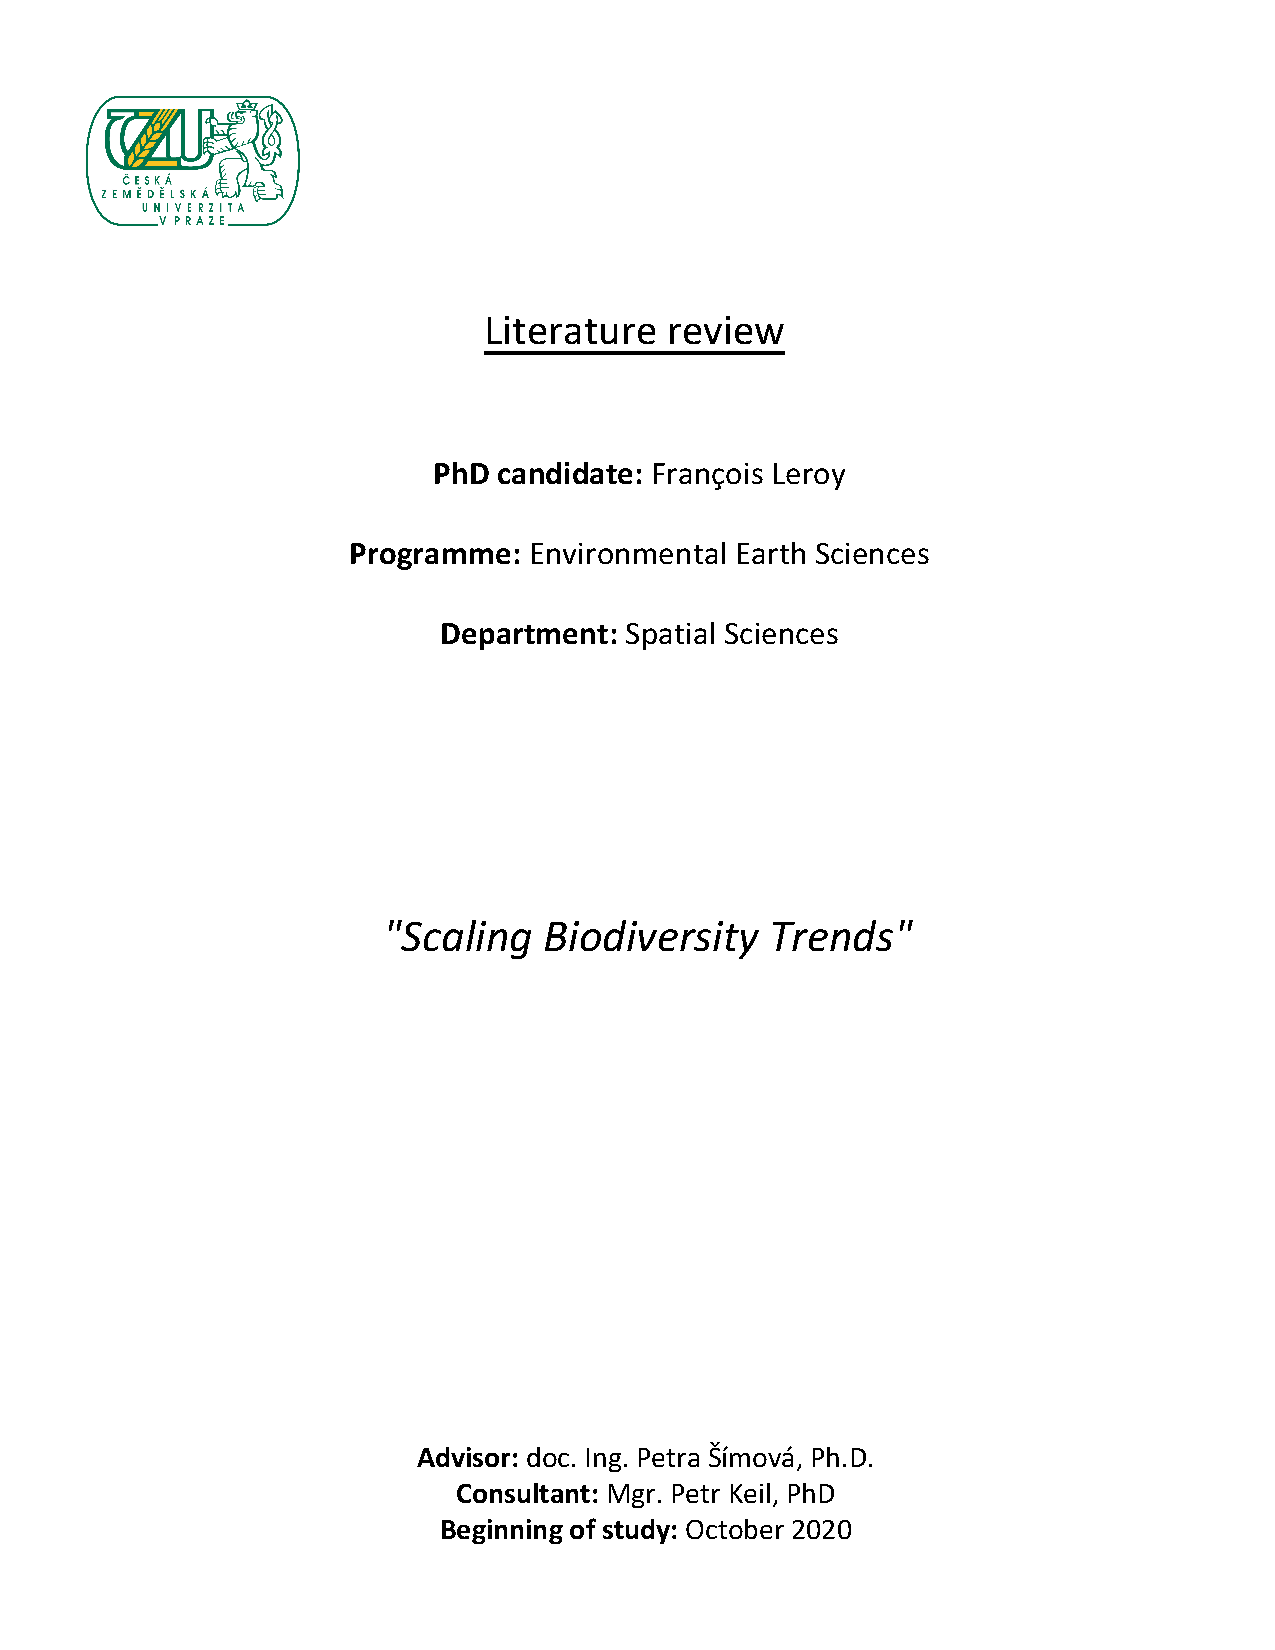
\includepdf[pages = {1}, fitpaper=true]{_assets/coverpage.pdf}

% Roman numbering for content before toc and toc itself
\cleardoublepage 
\pagenumbering{roman}

{
\hypersetup{linkcolor=}
\setcounter{tocdepth}{1}
\tableofcontents
\newpage
}
\vspace{50mm}
\setstretch{1.5}


% Start the arabic numbering at the 1st chapter
\cleardoublepage 
\pagenumbering{arabic}


% The mind, the...
\hypertarget{outline}{%
\chapter*{Outline}\label{outline}}
\addcontentsline{toc}{chapter}{Outline}

Literature review about the link between biodiversity facets trends and spatial/temporal scales.

The idea is to take every paper that talk about biodiversity trends (so far using just the species richness seems already a lot of paper) and to list \textbf{1)} which biodiversity metric they use \textbf{2)} which taxon/taxa they use, \textbf{3)} the spatial scale, \textbf{4)} the temporal scale and \textbf{5)} what is the dynamic (does the biodiversity metric increase/decrease/doesn't change over time/unclear).

Make a table of all these papers and \texttt{group\_by(taxa)\ \%\textgreater{}\%\ order\_by(spatial\_scale\ \textbar{}\ temporal\_scale)}. Then see if for each taxa we can find a trend (a bit like in Chase \emph{et al.} 2019 Oikos paper \textbar{} Jarzyna \emph{et al.} 2015 but here I am not making the analysis, just taking the analysis from papers). Best example found so far: \href{https://besjournals.onlinelibrary.wiley.com/doi/10.1111/j.0021-8901.2004.00926.x}{Hill \& Hamer 2004}

I am using the \enquote{Advanced Research} tab of Web of Science which allows me skim through the entire literature using a convenient syntax. For instance:

\begin{verbatim}
AB = ((biodiversity OR species richness OR diversity) AND
(temporal trend* OR dynamic*) AND
(bird* OR avia*)) 
\end{verbatim}

And

\begin{verbatim}
AB = ((biodiversity change index)  AND (bird*  OR avia*)  AND trend*)
\end{verbatim}

And

\begin{verbatim}
AB = ((species richness) AND (bird* OR avia*) AND trend*) 
\end{verbatim}

And

\begin{verbatim}
ALL=(birds AND species richness AND temporal trend)
\end{verbatim}

\hypertarget{dashboard}{%
\chapter*{Dashboard}\label{dashboard}}
\addcontentsline{toc}{chapter}{Dashboard}

\href{https://www.sciencedirect.com/science/article/pii/S1470160X20306658?via\%3Dihub}{Reference paper}

\begin{itemize}
\item
  05/07/2021: research wos made with the literature review filter for the first query (stopped at \#13) and created the second query (stopped at \#2)
\item
  07/07/2021: questions to Petr: \textbf{1)} can the geometric mean of relative abundance + the weighted goodness of fit be used as biodiversity trend index, \textbf{2)} can the Farmland Bird Indicator (FBI) be used as biodiversity trend (for me it is more biodiversity health, Chiron et al 2013) \textbf{3)} what about the Red List Index trend? \textbf{4)} what about Multispecies population indexes?
\item
  08/07/2021: stopped at the article 41 for research \#2.
\item
  12/08/2021: stopped at article 4 for research \#4
\item
  13/08/2021: stopped at article 8 for research \#4
\item
  17/08/2021: stopped at article 15 for research \#4
\item
  18/08/2021: stopped at article 30 for research \#4
\item
  19/08/2021: stopped at article 46 for research \#4
\item
  20/08/2021: stopped at article 64 for research \#4
\end{itemize}

\hypertarget{introduction}{%
\chapter{Introduction}\label{introduction}}

Human life quality is intrinsically linked to ecosystems state that he is living in. Indeed, ecosystems services extend in a large spectrum of mechanisms including nutrient cycle, food production, or climate and water cycle regulation \citep{pereira_global_2012}. Some of those ecosystem functions are managed by bird biodiversity such as seed dispersal, controls pests or pollinate plant. Unfortunately, anthropogenic stressors like habitat loss, over exploitation, pollution or introduction of invasive species could lead biodiversity to its sixth mass extinction \citep{barnosky_has_2011}.

Biodiversity erosion is now known from everyone and political decisions has been stated in order to limit it \citep[\emph{e.g.}][2010, 2002]{the_convention_on_biological_diversity_convention_2021}. However, these objectives have been so far not reached due mainly to our confusion and misunderstanding about biodiversity dynamic and how to determine it.

As a matter of fact, studying biodiversity can be confusing, especially because several choices must be done. Firstly, the level at which you are looking at the biodiversity must be chosen (\emph{e.g.} species, functional, phylogenetic diversity). Secondly, one must decide which metric is the most appropriate for his study. There are many facets of biodiversity that can be measured by different metrics depending on the objective of your study. Measures of static biodiversity are commonly used such as species richness or \(\alpha\) diversity \citep[\emph{i.e.} number of species,][]{whittaker_vegetation_1960}, the Shannon index \citep{shannon_mathematical_1948} ,the Simpson index \citep{simpson_measurement_1949} or the Hill number \citep{hill_diversity_1973}. The later three biodiversity indexes take into account the relative abundances of the species and can be considered as the \emph{quality} of the biodiversity. On an other hand, the spatial and temporal \(\beta\) diversity will measure the species turnover and can be measured thanks to Whittaker's \citep{whittaker_evolution_1972}, Sørensen's \citep{sorensen_method_1948} or Jaccard's \citep{jaccard_distribution_1912} dissimilarity indexes \citep[\emph{e.g.}][]{keil_patterns_2012}.

However, overall biodiversity (\emph{i.e.} taking into account species of every taxa) may not be relevant for one's case study. Thus, several multi-species indicators have also been created, taking into account the abundances of indicator species giving information on the ecosystem health. The most known ones are the Red List Index \citep{butchart_improvements_2007, butchart_using_2005, butchart_measuring_2004} or the Biodiversity Change Index \citep{normander_indicator_2012}.

Using all the metrics cited above, we now know that the loss of global biodiversity is unprecedented. However, current scientific literature has also shown that temporal trends in local changes of biodiversity can be opposite to trends at larger scales \citep[\emph{e.g.}][]{chase_species_2019}. Thus, current changes in biodiversity is far more complex than a simple global decrease: most of the ecosystems undergo alterations of their communities with changes in species composition \citep{blowes_geography_2019, dornelas_quantifying_2013}. Wonders persist about how the trend of these different metrics of biodiversity are link to the spatial and temporal scales used when measured.

In order to investigate this link between spatial scales and biodiversity metrics, birds is a relevant taxon. Thanks to the many ornithological monitoring and surveys, we now have a large number of long, high-quality time series on bird populations \citep{bejcek_velke_2016}. Birds are easy to observe, easy to identify and thus many volunteers are motivated to conduct standardized sampling. Given their ability to change quickly of locations, their presence is also a good indicator for ecosystem health and thus several standardized metrics have been created to assess their populations. For instance, the geometric mean of relative abundances or the goodness-of-fit statistic \citep{studeny_goodness_2011} are some of the baseline. Other multi-species indicators have also been created specifically for birds, such as the Farmland Bird Indicator \citep{gregory_developing_2005}, the Forest Bird Indicator \citep{gregory_population_2007} or the Wild Bird Indicator \citep{gregory_wild_2010}.

Here, I propose to review articles assessing the temporal trends of different avian biodiversity metrics and to look at which spatial scales these studies have been done. Summarizing the trends of these qualitative and/or quantitative avian biodiversity indexes along with their spatial and temporal scales will help to see more clearly how the trends of biodiversity are linked to spatio-temporal scales. It is also important to demonstrate that the information about the sampling plan (\emph{i.e.} spatial scale, time span, temporal scales etc) is not systematically indicated in the scientific literature and can bring confusion to the analysis and comparisons of their trends. I believe that this review can help to have a better overview of the current knowledge on the trend of biodiversity metrics of bird populations.

\hypertarget{materials-and-methods}{%
\chapter{Materials and Methods}\label{materials-and-methods}}

I used the \emph{\enquote{advanced serach}} tool of the ISI Web of Science Core collection database. It allowed me to write these four following queries using key words:

\begin{enumerate}
\def\labelenumi{\arabic{enumi}.}
\item
  \texttt{AB\ =\ ((biodiversity\ OR\ species\ richness\ OR\ diversity)\ AND\ (temporal\ trend*\ OR\ dynamic*)\ AND\ (bird*\ OR\ avia*))} which resulted in 1346 references.
\item
  \texttt{AB\ =\ ((biodiversity\ change\ index)\ \ AND\ (bird*\ \ OR\ avia*)\ \ AND\ trend*)} which resulted in 60 references.
\item
  \texttt{AB\ =\ ((species\ richness)\ AND\ (bird*\ OR\ avia*)\ AND\ trend*)} which resulted in 313 references.
\item
  \texttt{ALL=(birds\ AND\ species\ richness\ AND\ temporal\ trend)} which resulted in 88 references.
\end{enumerate}

\begingroup\fontsize{10}{12}\selectfont

\begin{longtable}[t]{l}
\caption{\label{tab:unnamed-chunk-3}SR = species richness, Ab = abundance, Eve = evenness, }\\
\toprule
Reference\\
\midrule
\endfirsthead
\caption[]{\label{tab:unnamed-chunk-3}SR = species richness, Ab = abundance, Eve = evenness,  \textit{(continued)}}\\
\toprule
Reference\\
\midrule
\endhead

\endfoot
\bottomrule
\endlastfoot
\cite{barnagaud_temporal_2017}\\
\cite{barnagaud_temporal_2017}\\
\cite{barnagaud_temporal_2017}\\
\cite{barnagaud_temporal_2017}\\
\cite{barnagaud_temporal_2017}\\
\addlinespace
\cite{barnagaud_temporal_2017}\\
\cite{roels_recovery_2019}\\
\cite{roels_recovery_2019}\\
\cite{wretenberg_changes_2010}\\
\cite{ram_what_2017}\\
\addlinespace
\cite{ram_what_2017}\\
\cite{ram_what_2017}\\
\cite{ram_what_2017}\\
\cite{ram_what_2017}\\
\cite{harrison_quantifying_2016}\\
\addlinespace
\cite{harrison_quantifying_2016}\\
\cite{harrison_quantifying_2016}\\
\cite{doxa_low-intensity_2010}\\
\cite{doxa_low-intensity_2010}\\
\cite{doxa_low-intensity_2010}\\
\addlinespace
\cite{arnold_contrasting_2021}\\
\cite{arnold_contrasting_2021}\\
\cite{arnold_contrasting_2021}\\
\cite{xu_detecting_2018}\\
\cite{jiguet_french_2012}\\
\addlinespace
\cite{jiguet_french_2012}\\
\cite{jiguet_french_2012}\\
\cite{keten_temporal_nodate}\\
\cite{davey_rise_2012}\\
\cite{davey_rise_2012}\\
\addlinespace
\cite{davey_rise_2012}\\
\cite{siriwardena_how_2019}\\
\cite{christian_more_2009}\\
\cite{dittrich_multiyear_2019}\\
\cite{dittrich_multiyear_2019}\\
\addlinespace
\cite{dittrich_multiyear_2019}\\
\cite{dittrich_multiyear_2019}\\
\cite{sirami_changes_2012}\\
\cite{garcia-navas_temporal_2020}\\
\cite{mcgeoch_global_2010}\\
\addlinespace
\cite{ellis_twenty-year_2019}\\
\cite{ellis_twenty-year_2019}\\
\cite{ellis_twenty-year_2019}\\
\cite{ellis_twenty-year_2019}\\
\cite{ellis_twenty-year_2019}\\
\addlinespace
\cite{ellis_twenty-year_2019}\\
\cite{ellis_twenty-year_2019}\\
\cite{ellis_twenty-year_2019}\\
\cite{ellis_twenty-year_2019}\\
\cite{ellis_twenty-year_2019}\\
\addlinespace
\cite{ellis_twenty-year_2019}\\
\cite{ellis_twenty-year_2019}\\
\cite{sicurella_effectiveness_2018}\\
\cite{sicurella_effectiveness_2018}\\
\cite{sicurella_effectiveness_2018}\\
\addlinespace
\cite{nally_monitoring_1997}\\
\cite{latta_patterns_2011}\\
\cite{latta_patterns_2011}\\
\cite{scarton_long-term_2017}\\
\cite{scarton_long-term_2017}\\
\addlinespace
\cite{scarton_long-term_2017}\\
\cite{scarton_long-term_2017}\\
\cite{chiron_forecasting_2013}\\
\cite{chiron_forecasting_2013}\\
\cite{chiron_forecasting_2013}\\
\addlinespace
\cite{chiron_forecasting_2013}\\
\cite{eglington_disentangling_2012}\\
\cite{harrison_assessing_2014}\\
\cite{harrison_assessing_2014}\\
\cite{harrison_assessing_2014}\\
\addlinespace
\cite{harrison_assessing_2014}\\
\cite{harrison_assessing_2014}\\
\cite{harrison_assessing_2014}\\
\cite{juslen_application_2013}\\
\cite{normander_indicator_2012}\\
\addlinespace
\cite{normander_indicator_2012}\\
\cite{normander_indicator_2012}\\
\cite{schipper_contrasting_2016}\\
\cite{schipper_contrasting_2016}\\
\cite{schipper_contrasting_2016}\\
\addlinespace
\cite{schipper_contrasting_2016}\\
\cite{schipper_contrasting_2016}\\
\cite{schipper_contrasting_2016}\\
\cite{schipper_contrasting_2016}\\
\cite{schipper_contrasting_2016}\\
\addlinespace
\cite{schipper_contrasting_2016}\\
\cite{schipper_contrasting_2016}\\
\cite{schipper_contrasting_2016}\\
\cite{schipper_contrasting_2016}\\
\cite{schipper_contrasting_2016}\\
\addlinespace
\cite{schipper_contrasting_2016}\\
\cite{schipper_contrasting_2016}\\
\cite{schipper_contrasting_2016}\\
\cite{schipper_contrasting_2016}\\
\cite{schipper_contrasting_2016}\\
\addlinespace
\cite{schipper_contrasting_2016}\\
\cite{schipper_contrasting_2016}\\
\cite{schipper_contrasting_2016}\\
\cite{schipper_contrasting_2016}\\
\cite{schipper_contrasting_2016}\\
\addlinespace
\cite{schipper_contrasting_2016}\\
\cite{schipper_contrasting_2016}\\
\cite{schipper_contrasting_2016}\\
\cite{schipper_contrasting_2016}\\
\cite{schipper_contrasting_2016}\\
\addlinespace
\cite{schipper_contrasting_2016}\\
\cite{schipper_contrasting_2016}\\
\cite{schipper_contrasting_2016}\\
\cite{schipper_contrasting_2016}\\
\cite{schipper_contrasting_2016}\\
\addlinespace
\cite{schipper_contrasting_2016}\\
\cite{schipper_contrasting_2016}\\
\cite{schipper_contrasting_2016}\\
\cite{schipper_contrasting_2016}\\
\cite{schipper_contrasting_2016}\\
\addlinespace
\cite{schipper_contrasting_2016}\\
\cite{schipper_contrasting_2016}\\*
\end{longtable}
\endgroup{}

\hypertarget{references}{%
\chapter*{References}\label{references}}
\addcontentsline{toc}{chapter}{References}

\singlespacing


  \bibliography{references.bib}

\end{document}
